\documentclass[openacc]{rstransa} %%%%where rstrans is the template name

\usepackage{amsfonts}
\usepackage{amsmath}
\usepackage{amssymb}
\usepackage{booktabs}
\usepackage{caption}
\usepackage{color}
\usepackage{comment}
\usepackage{float}
\usepackage{graphicx}
\usepackage{hyperref}
\usepackage[utf8]{inputenc} % allows using accents directly in text, like ÔøΩ
\usepackage{subfig}
\usepackage{xspace}
\usepackage{anyfontsize} % added to avoid font size replacement
\usepackage{multirow} 

\newcommand{\pygbe}{\texttt{PyGBe}\xspace}

\graphicspath{{figs/}} %  PATH to figure files-- change to ./ for submission


\begin{document}
%%%% Article title to be placed here
\title{Reproducible Validation and Replication Studies in Nanoscale Physics}

\author{%%%% Author details
N. C. Clementi$^{1}$, L. A. Barba$^{1}$}

%%%%%%%%% Insert author address here
\address{$^{1}$Department of Mechanical and Aerospace Engineering, 
The George Washington University, Washington D.C., USA }

%%%% Subject entries to be placed here %%%%
\subject{xxxxx, xxxxx, xxxx}

%%%% Keyword entries to be placed here %%%%
\keywords{xxxx, xxxx, xxxx}

%%%% Insert corresponding author and its email address}
\corres{L.A. Barba\\
\email{labarba@gwu.edu}}

%%%% Abstract text to be placed here %%%%%%%%%%%%
\begin{abstract}
    The abstract text goes here. 
\end{abstract}
%%%%%%%%%%%%%%%%%%%%%%%%%%%
    
%%%%%%%%%% Insert the texts which can accommodate on firstpage in the tag "fmtext" %%%%%
    
\begin{fmtext}  
\section{Introduction}

PUT SOMETHING HERE. I DON'T GET WHAT WE ARE SUPPOSE TO PUT HERE, BUT THE GUIDELINES HAVE THIS

\end{fmtext}

\maketitle
% Body of paper.
\section{Background and methods}\label{sec:background}
%!TEX root = ClementiBarba2020.tex

\subsection{Verification, validation, reproducibility and replication}

\subsection{Description of the PyGBe software}

\subsection{Physics context for this work}

\section{Results} \label{sec:results}
%!TEX root = ClementiBarba2020.tex
All the results reported in this paper were obtained using the \pygbe software \cite{ClementiETal2017},
with the version at commit \href{https://github.com/pygbe/pygbe/tree/e1f3650b0c99cab99dcfe5372200d3a1534eddfe}{34eddfe} in the history.
The software GitHub repository contains a Dockerfile to create the container image where we ran the simulations. 
The manuscript GitHub repository is separate from the software repository, and can be found at \url{https://github.com/barbagroup/pygbe_validation_paper}.
It contains the reproducibility packages for all results, as described in sub-section \ref{sec:reprod} and elsewhere in the paper.
We used a lab workstation for all simulations, built from parts.
Hardware specifications are as follows: 
\begin{compactitem}
  \item[$\triangleright$] CPU: Intel Core i7-5930K Haswell-E 6-Core 3.5GHz LGA 2011-v3
  \item[$\triangleright$] RAM: G.SKILL Ripjaws 4 series 32GB (4 x 8GB)
  \item[$\triangleright$] GPU: Nvidia Tesla K40c (with 12 GB memory)
\end{compactitem}

\paragraph{Solver parameters:} We used a GMRES exit tolerance of $1\times10^{-6}$ in the iterative solver for all our simulations. Details on the treecode and integration parameters (and others)
can be found within input files included in the manuscript GitHub repository as part of the reproducibility packages (``repro-packs'').


\paragraph{Run times:} We report detailed time logs together with the data of our simulations, as part of the repro-packs to accompany this paper. Here is a brief report.
For the result of the replication of Figure 14 of Rockstuhl et al., sub-section \ref{sec:replication1}, the total wall-clock time for producing each curve was approximately 11.6 hours, which is the result of computing
the extinction cross section for 175 wavelength cases, giving $\approx$4 minutes per run. In the case of the validation and replication of Figure 2a of Ellis et al., sub-section \ref{sec:replication2}, 
the total wall-clock time for producing the curve was approximately 2.3 hours, which is the result of computing
the extinction cross section for 208 wavelength cases, giving $\approx$40 seconds per run.


\subsection{Replication of results from Rockstuhl, et al., 2005}\label{sec:replication1}

%%% Rockstuhl work summary%%%%
The work of Rockstuhl et al.\cite{rockstuhl2005} studies the phonon-polariton response of silicon carbide (SiC)
nanoparticles using a two-dimensional (2D) boundary element method, 
previously developed in their group \cite{rockstuhl2003}. 
They analyzed ``cylindrical particles'' (where they extend in the third dimension to infinity) made of 6H-SiC, with varying cross-sections.
%%% Rockstuhl work summary%%%%
We decided to attempt to replicate one of the results presented on Fig.14 of their paper:
the scattering cross-section of a SiC rectangular cylinder for three different aspect ratios. 
To be well within our quasistatic approach ($\lambda > d$ where $d$ is the characteristic
dimension of the geometry), we chose the case with $a=672$ nm, $b=328$ nm.

\subsubsection{Differences in method, mesh and dielectric data}

\paragraph{Method:} The main difference between the original simulations and ours is that they solve a 2D problem with the 
full Maxwell equations, while we solve a 3D problem with the electrostatic approximation. 
We lack any information about their code implementations, discretization schemes, or solver.  
We computed extinction cross-section (scattering plus absorption) while Rockstuhl et al.\ present only scattering cross-section. 
But, since the quantity of interest is the wavelength at which the resonance modes occur, the results can be compared.

\paragraph{Mesh:} Rockstuhl et al.\ did not provide any details regarding the discretization of the geometries or 
parameters involved in the simulations.
We performed a grid-independence study as a form of solution verification, and to ensure that we are 
minimizing errors due to discretization. Rockstuhl et al.\ used a 2D geometry (infinite third dimension), while we treat the geometry in its full 3D representation.

\paragraph{Dielectric data:} The study uses 6H-SiC as material, and the authors obtained their data from a source that we
were not able to replicate. Instead we are using experimental data for 4h-SiC that was provided to us 
via private communications from the authors of Ellis et al.\cite{ellis2016}.  

\subsubsection{Grid-independence study}\label{sec:independence}

We performed a grid-independence study on a SiC cube of side $L=535$ nm submerged in air, under a 
constant electric field aligned with the $z$-axis (a similar setup to the square cylinder on Fig. 18 of 
Rockstuhl et al.\cite{rockstuhl2005}). 
Due to the nature of the geometry and its sharp edges, it was challenging to see proper convergence. 
We have completed grid-convergence analysis for this type of physics in a previous work, but using spherical geometries \cite{ClementiETal2019}. 
With that experience, and given the difficulty caused by sharp edges, we are content with studying grid-independence here instead.
Figure \ref{fig:cube535} shows the grid-independence study, using meshes with  15,552 triangles (density $9.05\times10^{-4}$ per $\text{\AA}$ squared)
 to 19,200 triangles (density $1.11\times10^{-5}$ $\text{\AA}$ squared):
 the computed results show no discernible difference.

\begin{figure}
    \centering
    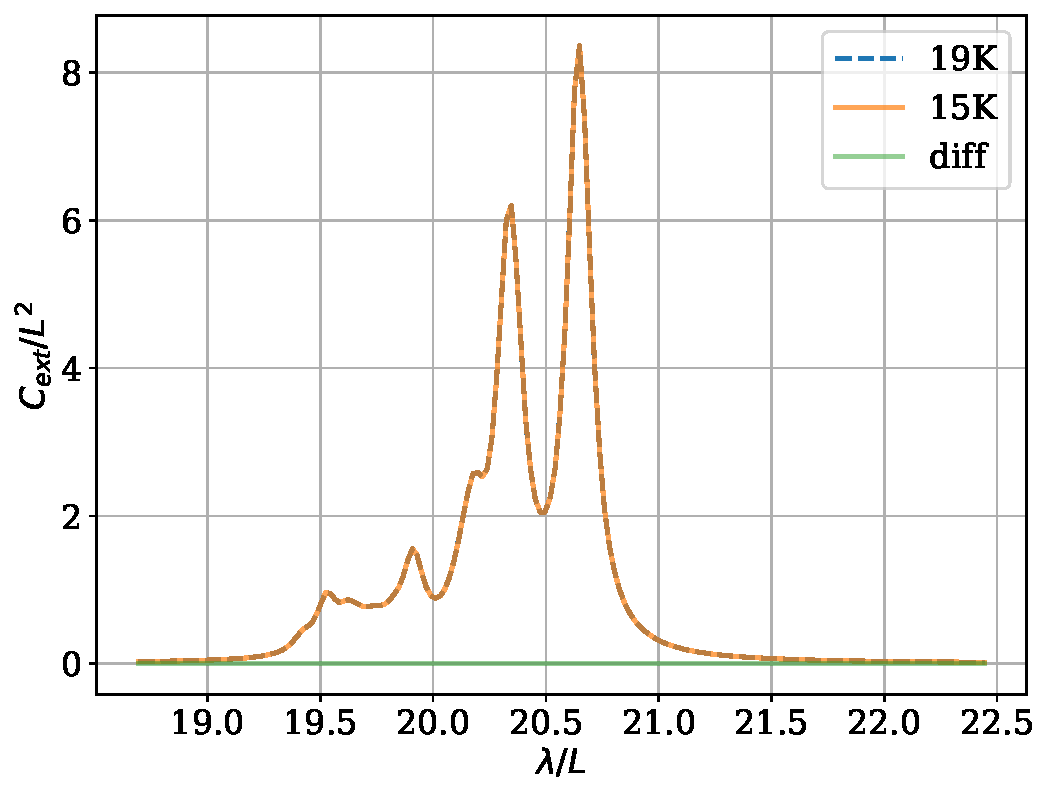
\includegraphics[width=0.75\textwidth]{cubeL535nm_15Kvs19K.pdf} 
    \caption{Grid-independence study for a SiC cube of side $L=535$ nm submerged in air under a constant 
    electric field in the $z$-direction. The curves represent the extinction cross-section divided by $L^2$ 
    as a function of wavelength divided by $L$, for mesh sizes 19K = 19,200 triangles and 15K = 15,552 triangles. 
    The label "diff" refers to the difference between the results of the two meshes.}
    \label{fig:cube535}
 \end{figure}

It is worth noting that the extinction cross-section curve in Figure \ref{fig:cube535} has extra peaks 
compared to the results of Figure 18 of Rockstuhl et al., due to the three-dimensional effects captured in our simulation and the sharp 
edges, the latter effect also being mentioned by Rockstuhl et al. The 3D effects will be approached
in the following results, where we attempt a replication of one of the results on Figure 14 of Rockstuhl et al. 

\subsubsection{Replication of Figure 14 (case a1) of Rockstuhl et al., 2005}

We chose to replicate a result of Rocksuthl et al.\ presented in Figure 14: 
the case where $a=672$ nm 
and $b=328$ nm, since these dimensions are well within the limits of the quasistatic approximation 
used in \pygbe. Rockstuhl et al.\ present the normalized scattering cross-section of a SiC rectangular 
cylinder, and they perform simulations for two different setups, sketched in Figure \ref{fig:rectangle_sketch}. In 
their Figure 14 (left), they have the wave vector (illumination) along the long 
side of the geometry, which means that the electric field is parallel to the short side of the rectangle, like in 
Figure \ref{fig:rectangle_sketch} (B). Following a similar analysis, in Figure 14 (right) of Rockstuhl et al., they have the wave 
vector (illumination) along the short side of the geometry, which means that the electric field is parallel to the 
long side of the rectangle, like in Figure \ref{fig:rectangle_sketch} (A). 

The constraints of mesh generation mean that we have only loose control on triangle density. Our meshes for the rectangular prism all have densities like in the coarse case of the grid-independence study of sub-section \ref{sec:independence}, or finer.
For the third dimension, we needed to choose a value that represents ``infinity.'' To achieve this, we studied the effects of 
elongating the cylinder to the third dimension. In Figure \ref{fig:ext_y_14}, we present the results for two different
values of the length in the third dimension, $y=1344$ nm ($2\times a$) and $y=2688$ nm ($4\times a$). We see that as we make $y$ longer, the 
intensity of some peaks decreases, due to the fact that some of the peaks are associated to this component. Therefore, 
from now on we use $y=2688$ nm. It is worth mentioning that the elongation of $y$ is limited to comply with the quasistatic limit, for this reason we have not explore bigger values of $y$.


\begin{figure}
    \centering
    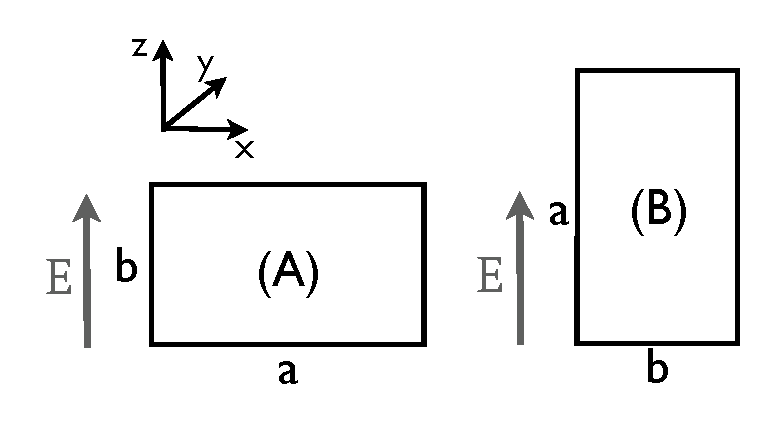
\includegraphics[width=0.45\textwidth]{rockstuhl_rectangles.pdf} 
    \caption{Configurations for the simulations corresponding to Fig. 14 of Rockstuhl et al., 2005.}
    \label{fig:rectangle_sketch}
\end{figure}

\begin{figure}
    \centering
    \subfloat{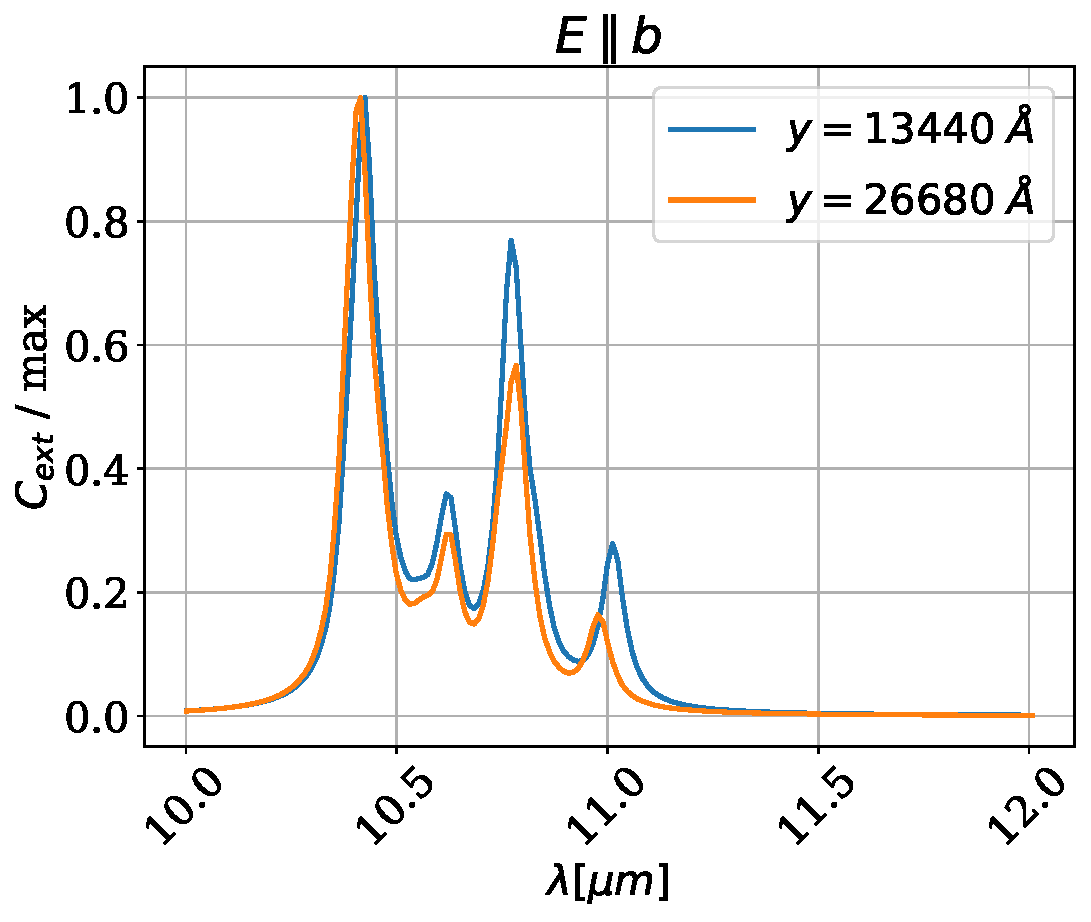
\includegraphics[width=0.48\textwidth]{ext_y_14a.pdf}}
    \subfloat{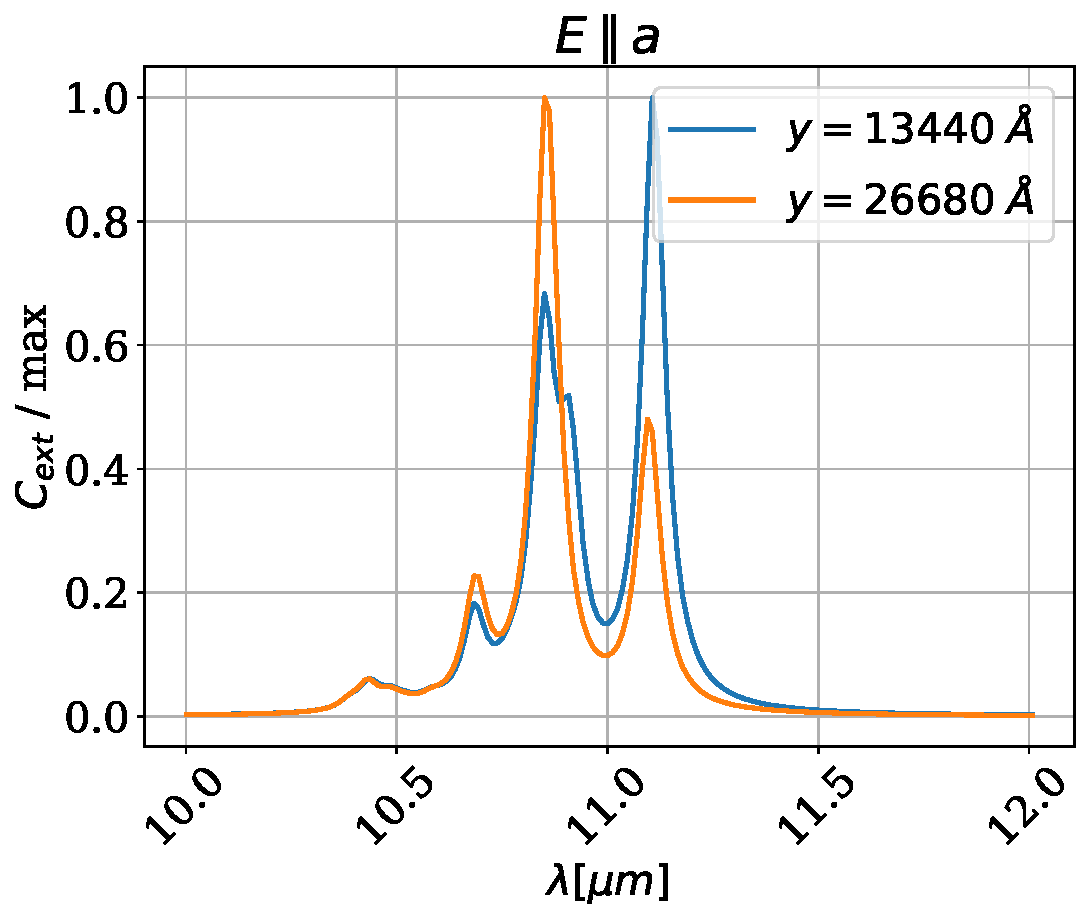
\includegraphics[width=0.48\textwidth]{ext_y_14b.pdf}} 
    \caption{Effect of the elongation of the third dimension ($y$) on the 
        extinction cross-section of a rectangular prism of SiC of dimensions $a=672$ nm 
        and $b=328$ nm, submerged in air and under a constant electric field 
        parallel to the $z$-axis. The left plot corresponds to a configuration such that the electric 
        field is parallel to $b$ (configuration (A) on Figure \ref{fig:rectangle_sketch}), while the 
        right plot corresponds to a configuration such that the electric field is 
        parallel to $a$ (configuration (B) on Figure \ref{fig:rectangle_sketch}.}
    \label{fig:ext_y_14}   
 \end{figure}


To generate the meshes for these simulations, we initially used the open source software Trimesh 
(\url{https://github.com/mikedh/trimesh}), but we realized that it was not producing a 
uniform mesh and that it was not possible to obtain regular triangles with the functions 
available when having a prism. To overcome this, we created our own mesh using Python scripts,
and obtained uniform meshes. We wanted to study the effect of a uniform mesh as well as the effect
of rounding the edges---Rockstuhl et al.\ mentioned rounded edges
as a factor that introduces extra peaks on the response. We were unable to control the 
roundness as a function of arc of curvature or the dimensions of the rectangular prism, so we 
decided to use the default settings on Trimesh. 
For reproducibility purposes, we provide all the mesh files, as described in sub-section \ref{sec:reprod}.
Figure \ref{fig:tri_reg_round_14} shows the 
results of the effect of uniformity and roundness. One can see that the second peak located at $\approx$ 10.6 $\mu$m  is much diminished in the green curve for both the $E\parallel b$  the $E\parallel a$ plots. 
These effects can be attributed 
to the effect of the roundness. This is consistent with the results in Rockstuhl et al. 

\begin{figure}
    \centering
    \subfloat{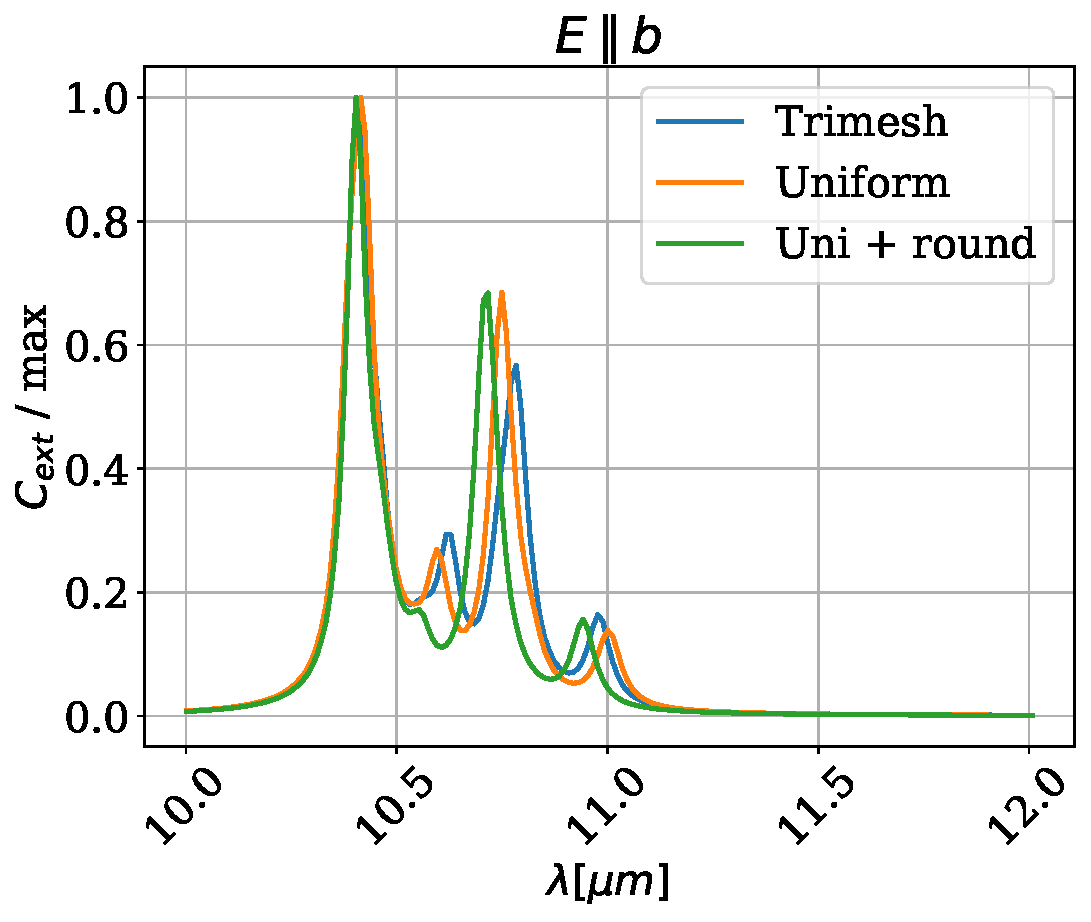
\includegraphics[width=0.48\textwidth]{tri_reg_round_14a.pdf}}
    \subfloat{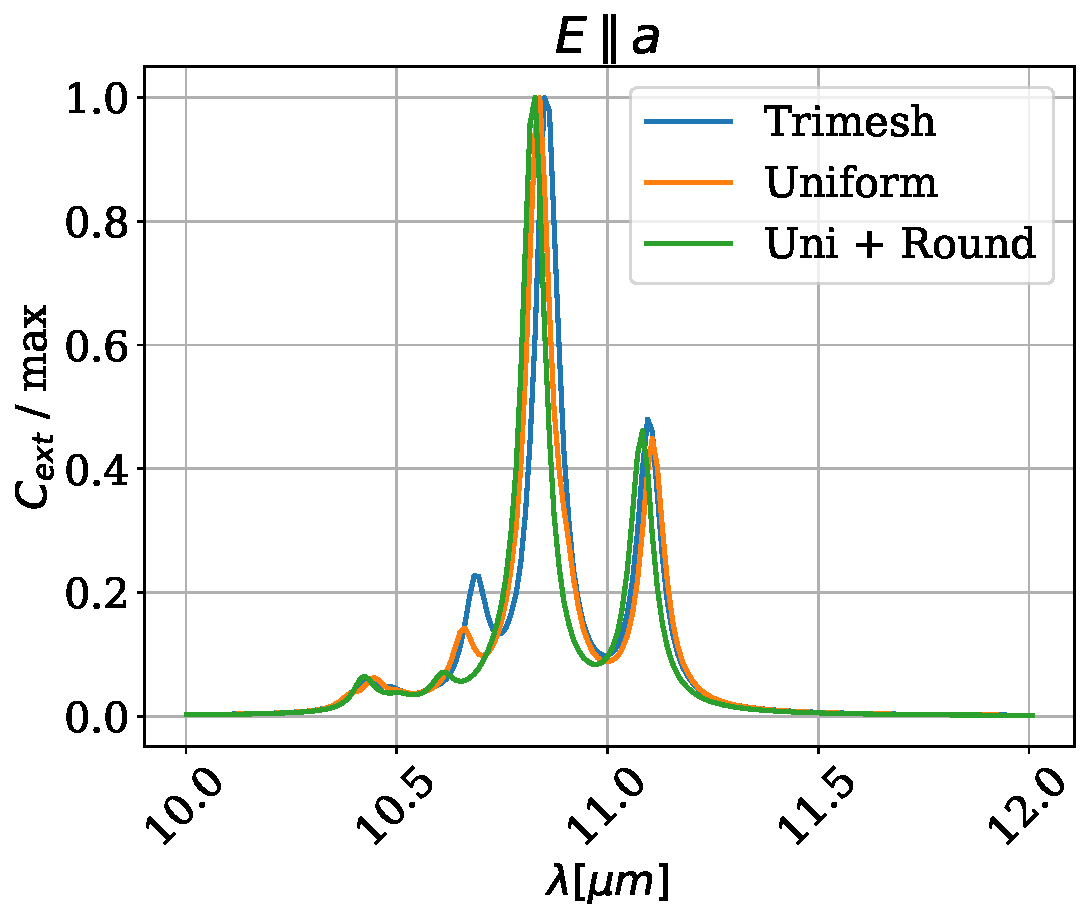
\includegraphics[width=0.48\textwidth]{tri_reg_round_14b.pdf}}
    \caption{Effect of uniformity of the mesh and roundness of the edges on the 
    extinction cross-section of a rectangular prism of SiC of dimensions $a=672$ nm, 
    $b=328$ nm and $y=2688$ nm, submerged in air and under a constant electric field 
    parallel to the $z$-axis. The labels are: \textbf{Trimesh}, for a non-uniform mesh generated using Trimesh; 
    \textbf{Uniform}, for a uniform mesh generated using Python scripts; and 
    \textbf{Uni + round}, for a uniform mesh generated using Python scripts with round 
    edges obtained using Trimesh.}
    \label{fig:tri_reg_round_14}
 \end{figure}

Once we have found the ``best'' possible geometry construction, we show how our results 
(green curve in Figure \ref{fig:tri_reg_round_14}) compare 
with the original results from Rockstuhl's Figure 14. We obtained data from Rockstuhl's curves by hand using 
the WebPlotDigitizer (\url{https://apps.automeris.io/wpd/}). The replication results are 
presented in Figure \ref{fig:rep_14}: the main resonance peaks presented in Rockstuhl et al.\ are 
closely matched. While we still have the presence of a third peak in our results, we conjecture 
that this is a consequence of the 3D effects in our geometry.

 \begin{figure}
    \centering
    \subfloat{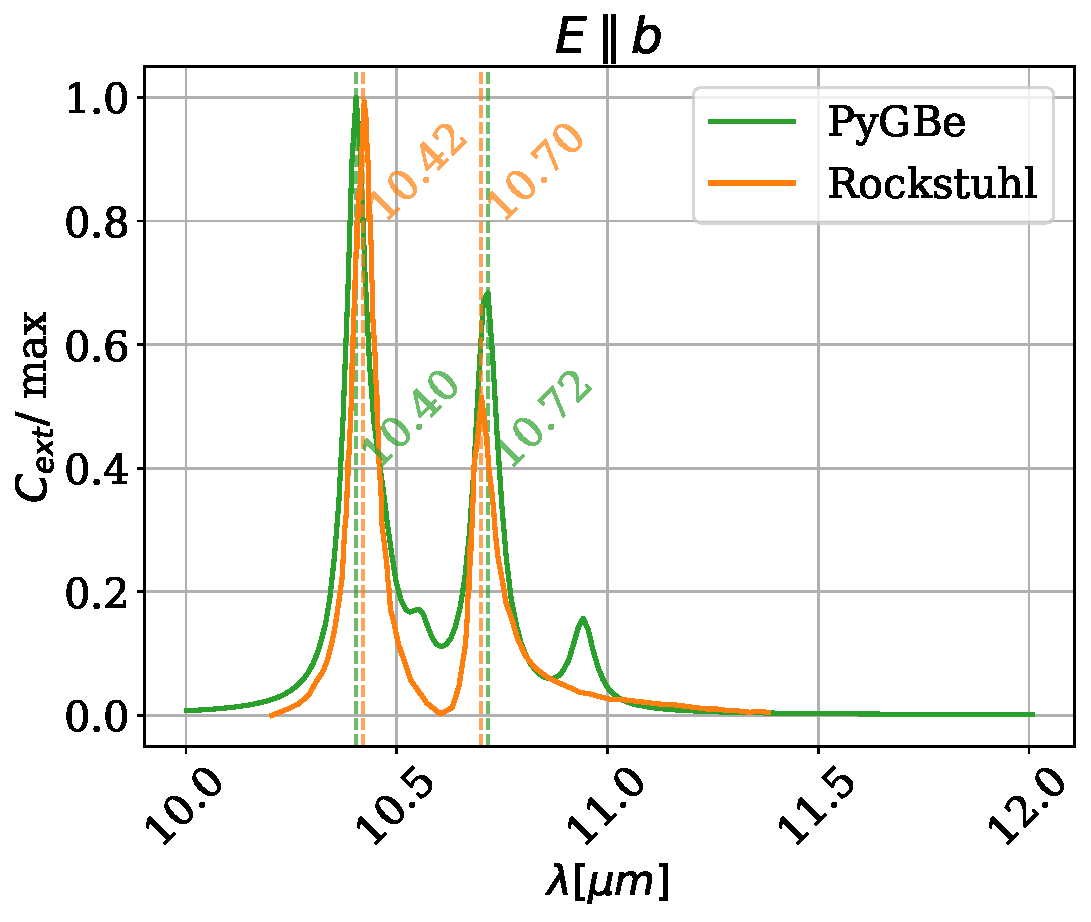
\includegraphics[width=0.48\textwidth]{replication_14a.pdf}}
    \subfloat{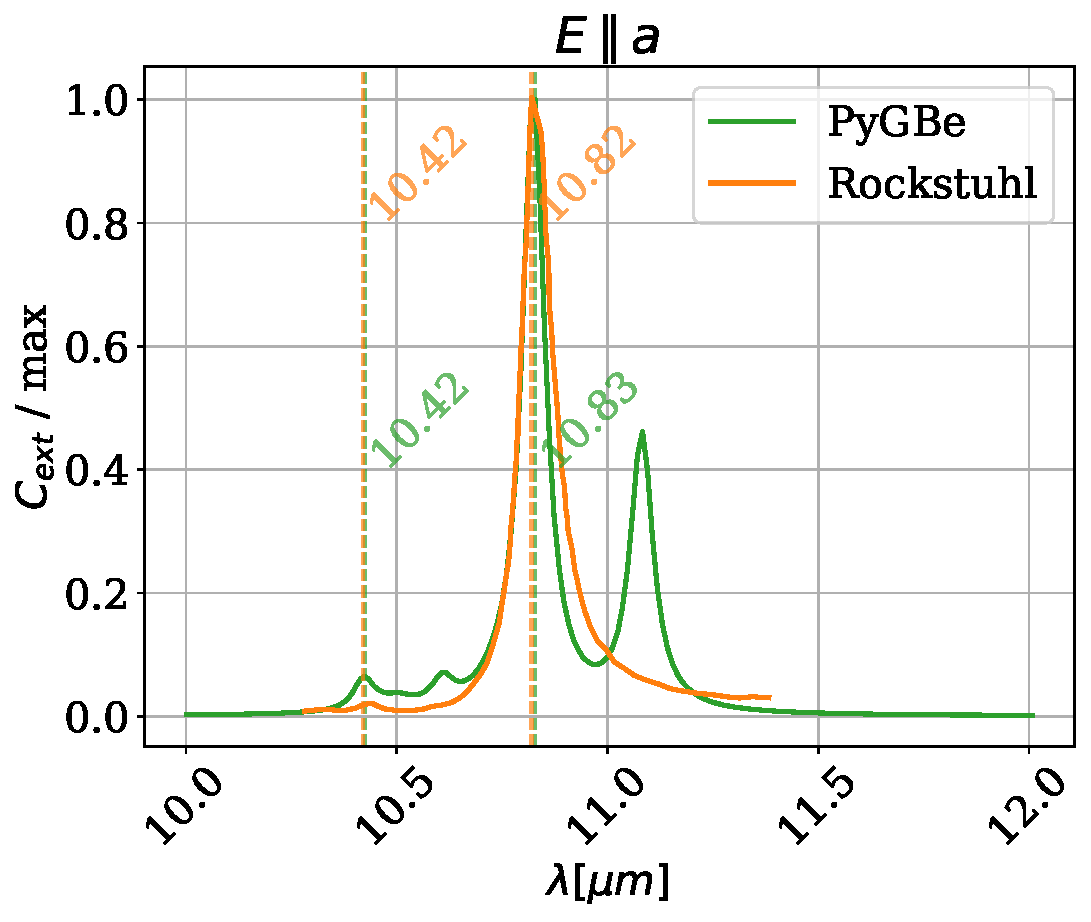
\includegraphics[width=0.48\textwidth]{replication_14b.pdf}} 
    \caption{Replication of the results in Figure 14 of Rockstuhl et al., 2005. Extinction cross-section of a
    rectangular prism of SiC of dimensions $a=672$ nm, $b=328$ nm and $y=2688$ nm, submerged
    in air and under a constant electric field parallel to the $z$-axis.}
    \label{fig:rep_14}
 \end{figure}


 \subsection{Replication of results from Ellis et al., 2016, and validation}\label{sec:replication2}

 %%% Ellis work summary %%%%
The work of Ellis and coworkers \cite{ellis2016} studies the aspect-ratio evolution of high-order
modes in localized surface phonon-polariton nanostructures. They study the
excitation of multipolar localized surface phonon polaritons (SPhP) resonances, by measuring
and computing polarized reflectance on 4H-SiC pillars of fixed height ($H=950$ nm), fixed 
width ($W=400$ nm) and varied length ($L=400$--$4800$ nm). These pillars are patterned on a square 
grid with a pitch $P=L+500$ nm to reduce coupling. In both their simulations and experiments, they 
measured polarized reflectance with the incident polarization 
oriented parallel or perpendicular to the long axis of the pillars.  
 %%% Ellis work summary %%%%

Our first aim was to replicate the computational result presented in Figure S4 of their supplementary 
material, corresponding to the black curve on their plot. In this 
figure, they show simulation results for the resonance spectral position of the lower-frequency 
mode when having parallel polarization ($E^{\parallel}_{100}$), with an incidence angle of 22$^\circ$.
We attempted to replicate this result since the gap between the pillars 
is 5000 nm (10 times larger than in the other cases), diminishing the effects of coupling, which makes it 
a better candidate to replicate using \pygbe. 
In our calculations, the setup consists of a single pillar, with no substrate.
Our second attempted replication is  
for the results presented in Figure 2a, corresponding to reflectance measurements across wave number
for pillars with aspect ratio $AR=4$, angle of incidence of 22 degrees, and incoming polarization parallel to the 
length of the pillars. For this case, the authors also reported experimental results that we will use for validation of our solver. 

\subsubsection{Differences in method, mesh and dielectric data}

\paragraph{Method:}
Ellis et al.\ ran experiments using reflectance spectroscopy and they computed the solution of
Maxwell's equations via the RF package of the finite element solver in the commercial software COMSOL. 
In their simulations, 
they used one pillar over a portion of substrate, with periodic boundary conditions to represent an array of 
pillars and their interactions. 
We use the boundary element method in the quasistatic approximation, which is suitable in this case 
since the pillar's size is small compared to the wavelengths involved in the simulations: 
which are in the range 10000--12500 nm. 
We measure extinction cross section, which will express as peaks instead of dips (shown in the reflection plots of Ellis et al.). 
The intensity of the peaks is not comparable, but we are looking to match the wave number (quantity of interest) at which these events happen. 

\paragraph{Mesh:}
For the case with aspect ratio $AR=4$, we have a non-uniform triangular surface mesh ($N=4398$) provided to us by the authors of 
Ellis et al., which we used for validation and replication of Figure 2a of their paper. However, for the replication
of Figure S4 of the supplementary material, we needed the remaining aspect ratio meshes. We generated uniform meshes using our
Python script, and we determined the density of these meshes by comparing the extinction cross section for the case with $AR=4$ of 
our mesh and the one provided by Ellis et al. We noticed that using around double the elements ($N=8564$) than in the original mesh and 
rounding the edges, the relative errors for the extinction cross section were, on average, smaller than 3$\%$, and the variation on the wavelength peak
position was smaller than 1 cm$^{-1}$. This analysis led us to a mesh density of $\approx \; 1.7 \times10^{-5}$ triangles per $\text{\AA}$ squared to create the meshes for 
the aspect ratio variation study.


\paragraph{Dielectric data:}
The dielectric data for the simulations was given to us by the authors of the paper via a private communication, 
and corresponds to experimental values of the dielectric. 

\subsubsection{Replication of Figure S4 in the supplementary materials of Ellis et al., 2016}

To be able to replicate the result of Figure S4 of the supplementary materials of Ellis et al., we
need to identify the lower-frequency mode for each of
the aspect ratios in our computations. For each aspect ratio ($AR$) 
value from 1 to 7, we computed the extinction cross section $C_{ext}$ across the wave numbers in the range
800--1000 cm$^{-1}$. We identified the lower-frequency mode ($E^{\parallel}_{100}$ for Ellis et al.) that is not a 
longitudinal mode. The longitudinal modes appear only when we have an incidence angle that is off-normal, since 
they are associated with the height of the pillar. Figure \ref{fig:AR_22_vs_norm} shows the results of the extinction 
cross-section of a SiC pillar of fixed height ($H=950$ nm), fixed width ($W=400$ nm) and varied length ($L=400$--$2800$ nm), for normal 
and 22-degrees angle of incidence. The simulations where performed 
for the long-edge orientation, meaning that the electric field is aligned with the length of the pillar 
when having normal incidence as shown on Figure \ref{fig:ellis_ang_inc}. From these results, we selected 
the lowest mode that it is not a longitudinal one and extracted its wavelength (see \ref{tab:ar_peaks}) to replicate 
\ref{fig:rep_FS4_ellis}. Figure \ref{fig:rep_FS4_ellis} shows the results from  Ellis et al. (digitized by hand using the WebPlotDigitizer) and the results obtained
with \pygbe, and Table \ref{tab:err_AR} shows that the percentage error is below 2$\%$ for all cases.
(Note that Ellis et al.\ changed the angle of incidence of the illuminating vector while in \pygbe we 
rotated the geometry instead.) 

\begin{figure}
    \centering
    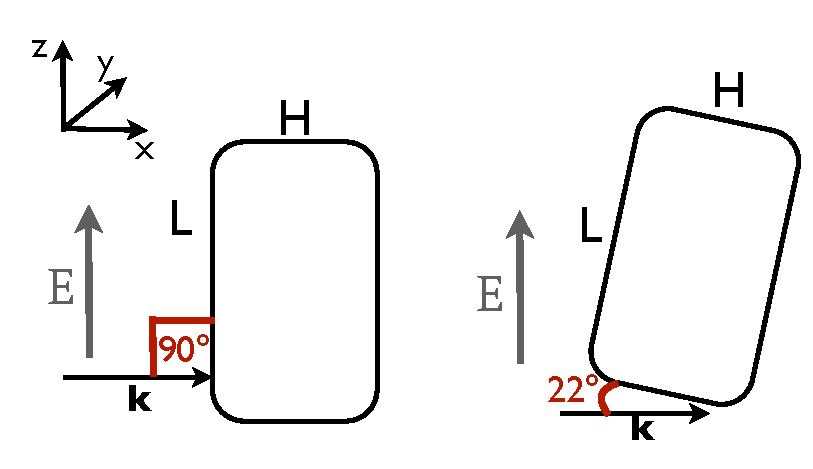
\includegraphics[width=0.45\textwidth]{ellis_ang_inc.pdf} 
    \caption{Diagram showing the angles of incidence in our simulation setups to comply with the configuration in the case from Ellis et al.}
    \label{fig:ellis_ang_inc}
 \end{figure}


\begin{figure}
    \centering
    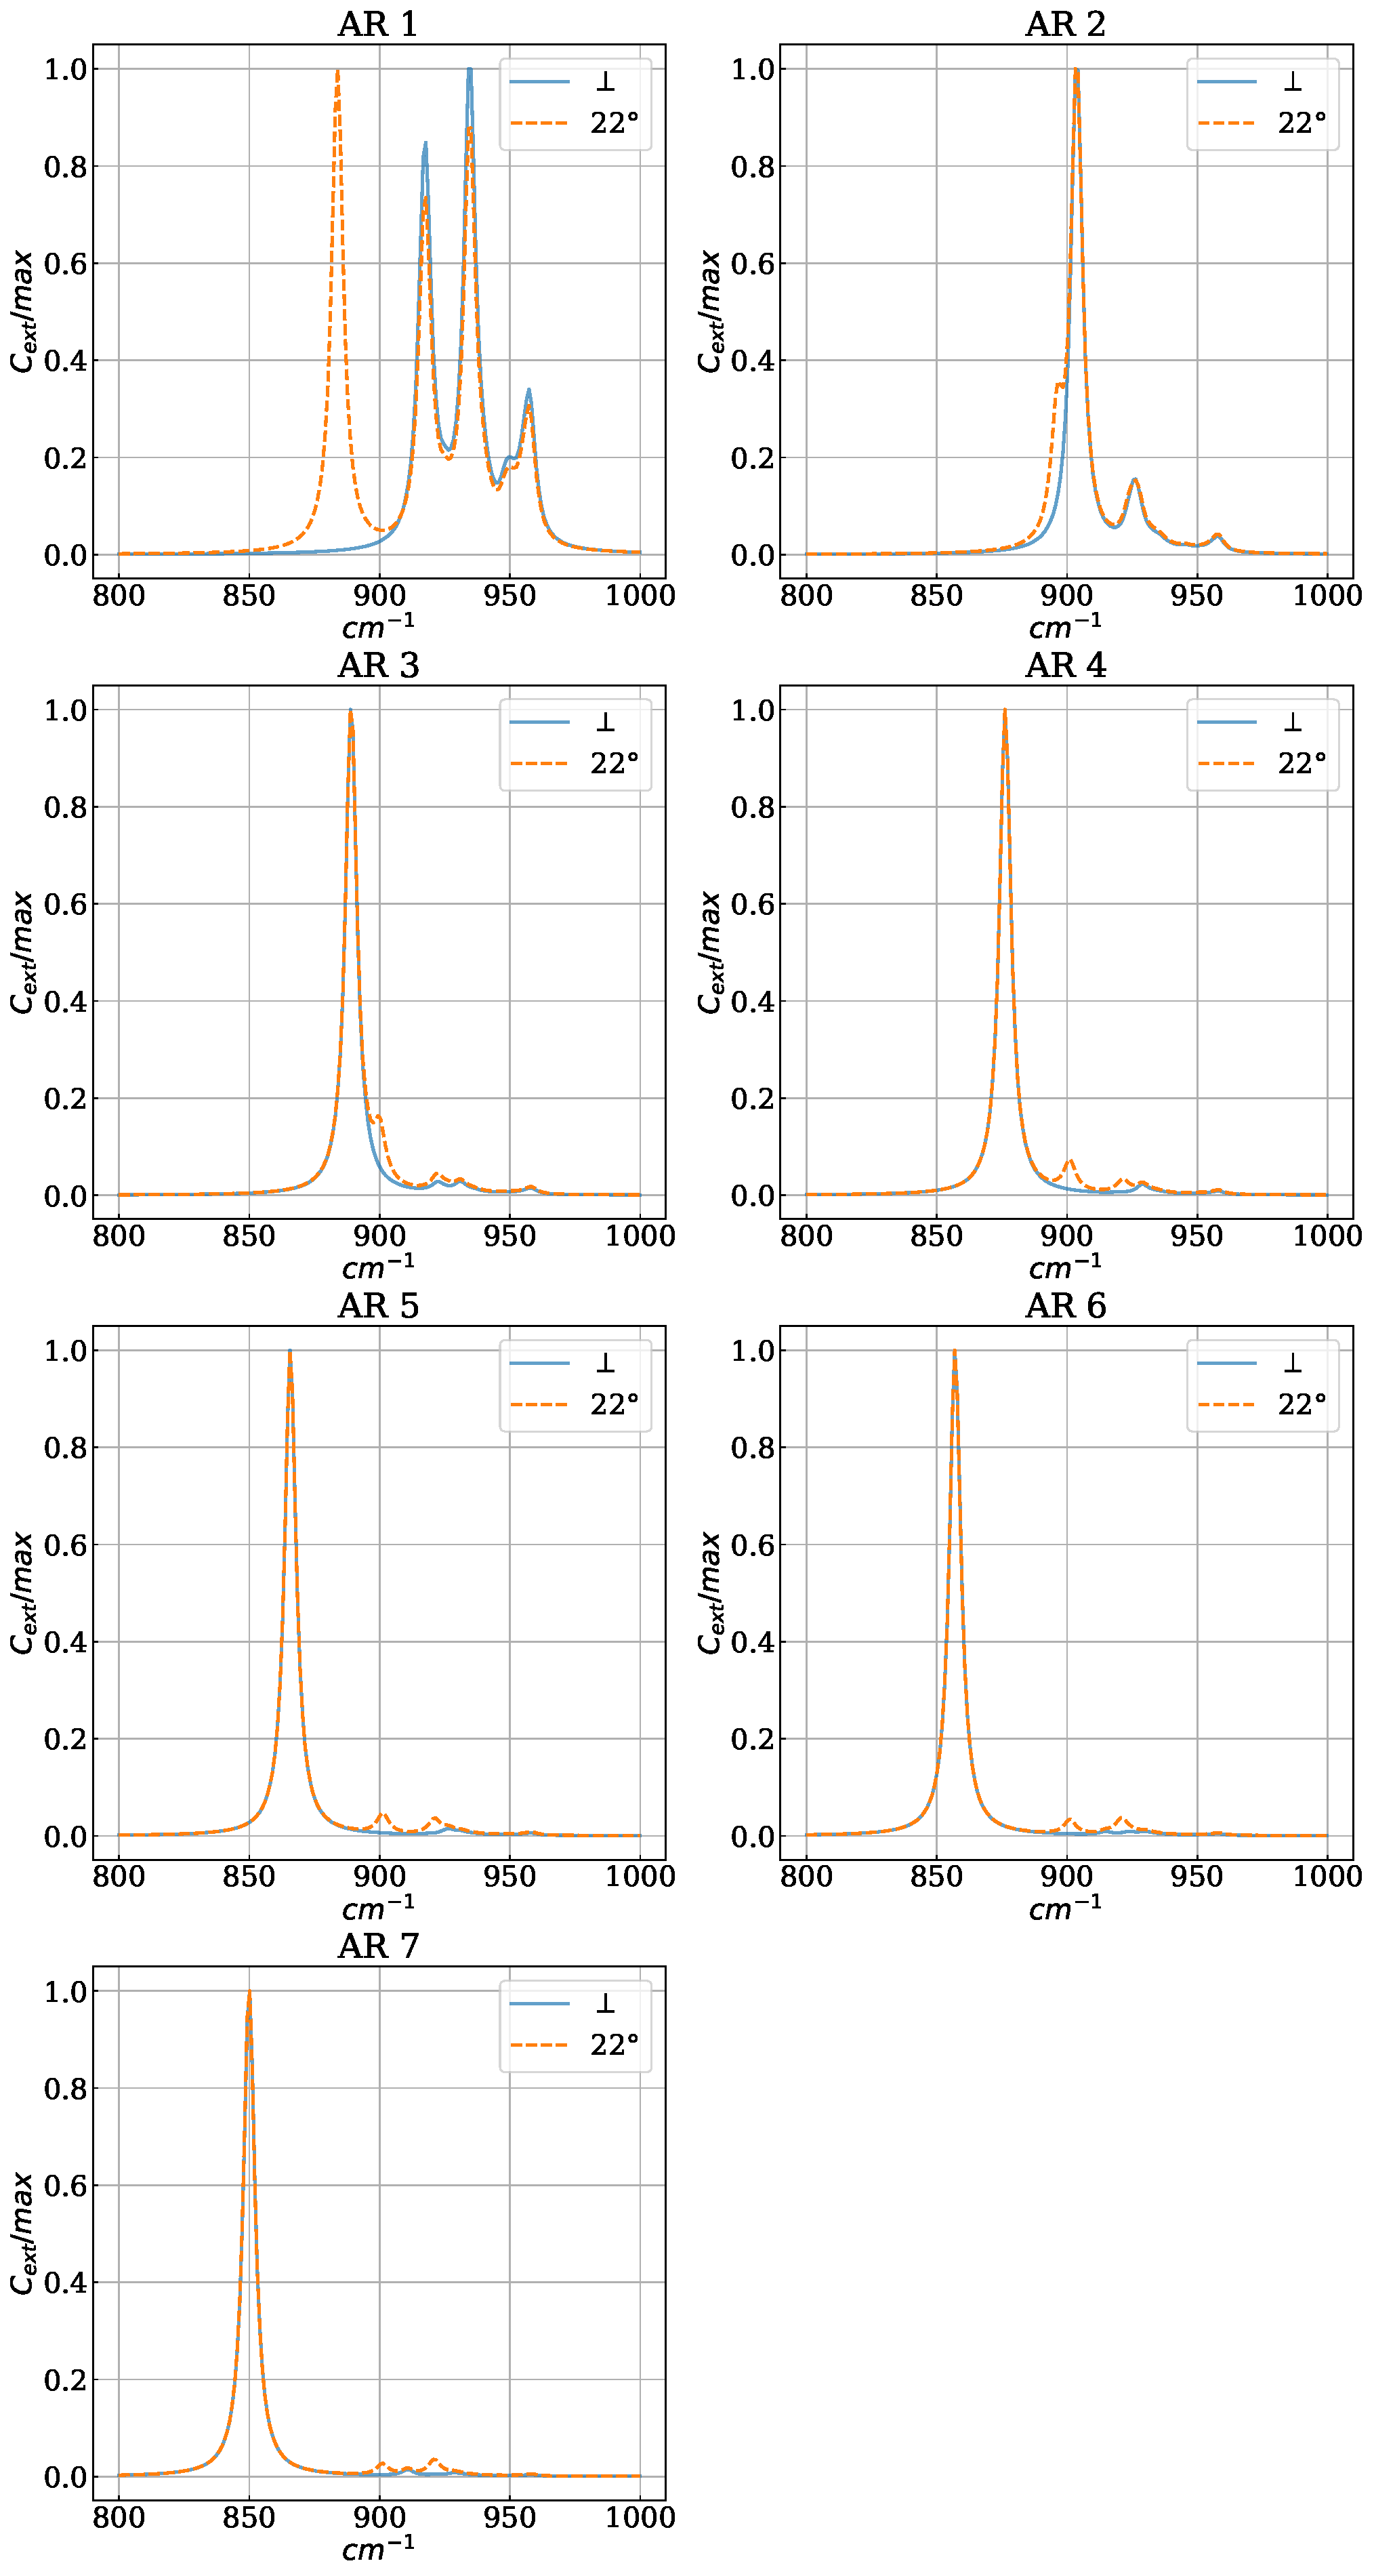
\includegraphics[width=0.8\textwidth]{AR_22_vs_norm.pdf} 
    \caption{Extinction cross-section across wavenumbers for SiC pillars of varying aspect ratios,  
             ($H=950$ nm, $W=400$ nm, $L=400$--$2800$ nm, $AR=1$--$7$), with both normal incidence and a 
             22-degree incidence.
            }
    \label{fig:AR_22_vs_norm}
 \end{figure}


\begin{table}
    \begin{center}
      \caption{Wavelength at which peaks happen for different aspect ratios, for runs where the electric
      field is parallel to the length ($L$) of the pillar. We have normal incidence and 22-degree incidence.}
      \label{tab:ar_peaks}
      \begin{tabular}{c c c c c c c c}
        \textbf{AR} \\
        \hline
        \multirow{2}{*}{1} & $\perp$ & \textbf{917.73} & 934.092 & 949.604 & 957.325 \\ % <-- Combining 2 rows with arbitrary with (*) and content 12
        & 22$^{\circ}$ & 883.926 & \textbf{917.73} & 935.052 & 949.604 & 957.325 \\ % <-- Content of first column omitted.
        \hline
        \multirow{2}{*}{2} & $\perp$ & \textbf{903.233} & 926.395 & 944.762 & 958.242 \\ % <-- Combining 2 rows with arbitrary with (*) and content 12
        & 22$^{\circ}$ & 896.517 & \textbf{903.233} & 926.395 & 944.762 & 958.242 \\ % <-- Content of first column omitted.
        \hline
        \multirow{2}{*}{3} & $\perp$ & \textbf{888.793} & 922.552 & 931.223 & 948.613 & 958.242 \\ % <-- Combining 2 rows with arbitrary with (*) and content 12
        & 22$^{\circ}$ & \textbf{888.793} & 899.418 & 922.552 & 931.223 & 958.242 \\ % <-- Content of first column omitted.
        \hline
        \multirow{2}{*}{4} & $\perp$ & \textbf{876.186} & 929.32 & 946.639 & 958.242 \\ % <-- Combining 2 rows with arbitrary with (*) and content 12
        & 22$^{\circ}$ & \textbf{876.186} & 901.281 & 921.618 & 929.32 & 945.745 & 958.242 \\ % <-- Content of first column omitted.
        \hline
        \multirow{2}{*}{5} & $\perp$ & \textbf{865.576} & 926.395 & 945.745 & 958.242 \\ % <-- Combining 2 rows with arbitrary with (*) and content 12
        & 22$^{\circ}$ & \textbf{865.576} & 901.281 & 921.618 & 958.242 \\ % <-- Content of first column omitted.
        \hline
        \multirow{2}{*}{6} & $\perp$ &  \textbf{856.904} & 914.793 & 923.489 & 929.32 & 946.639 & 958.242\\ % <-- Combining 2 rows with arbitrary with (*) and content 12
        & 22$^{\circ}$ & \textbf{856.904} & 901.281 & 920.6 & 958.242\\ % <-- Content of first column omitted.
        \hline
        \multirow{2}{*}{7} & $\perp$ &  \textbf{850.134} & 910.963 & 921.618 & 928.372 & 946.639 & 958.242 \\ % <-- Combining 2 rows with arbitrary with (*) and content 12
        & 22$^{\circ}$ & \textbf{850.134} & 901.281 & 910.963 & 920.6 & 958.242\\ % <-- Content of first column omitted.
        \hline
      \end{tabular}
    \end{center}
  \end{table}



\begin{figure}
    \centering
    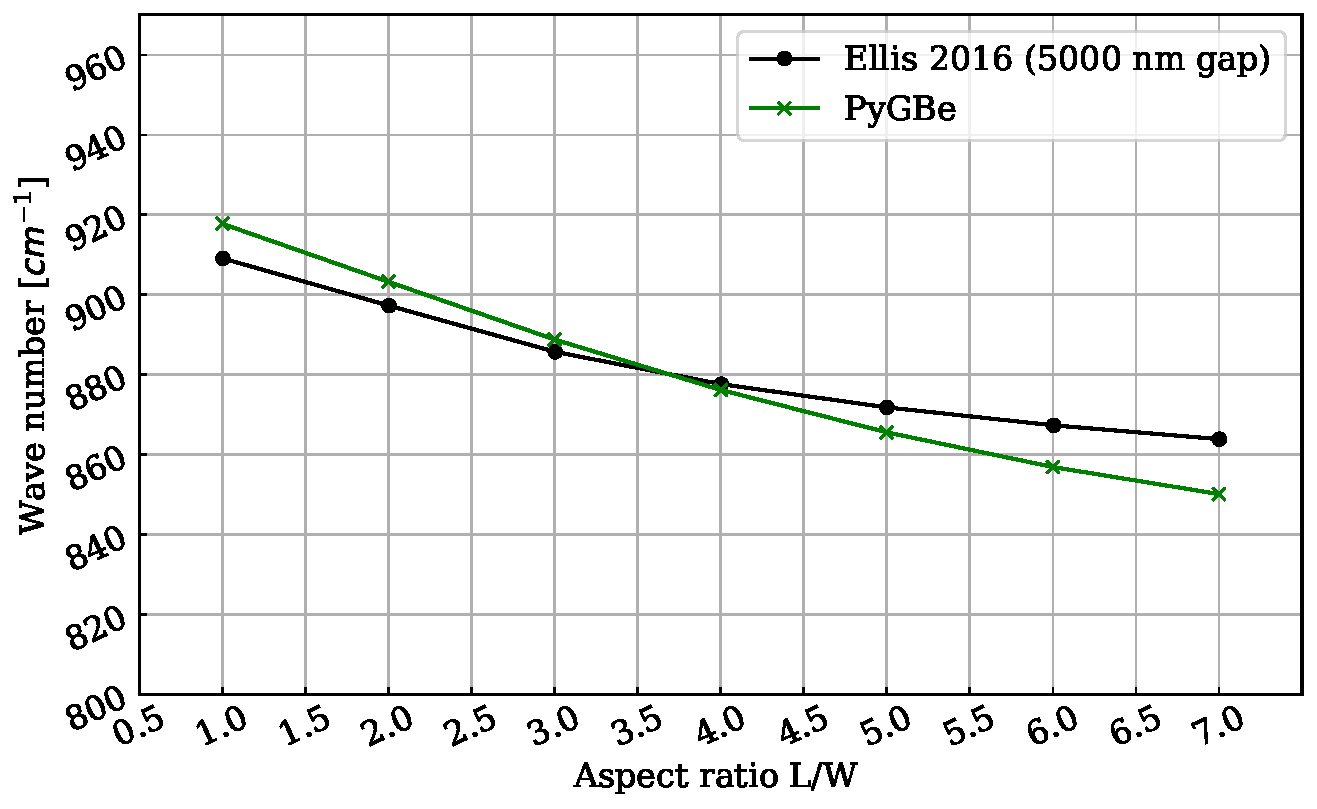
\includegraphics[width=0.85\textwidth]{AR_rep_FS4_Ellis2016.pdf} 
    \caption{Replication of figure S4 in the supplementary materials of Ellis et al., 2016. Wave
    number at which the $E^{\parallel}_{100}$ mode happens for different aspect ratios.}
    \label{fig:rep_FS4_ellis}
 \end{figure}
 
 \begin{table}
    \centering
    \caption{Percentage error for different aspect ratios.} 
    \label{tab:err_AR}
    \begin{tabular}{c c}
    \hline%\toprule
    AR & \% error \\
    \hline%\midrule
     $1$ & $0.95$ \\
     $2$ & $0.67$ \\
     $3$ & $0.35$ \\
     $4$ & $0.16$ \\
     $5$ & $0.72$ \\
     $6$ & $1.20$ \\
     $7$ & $1.59$ \\
    \hline%\bottomrule
    \end{tabular}
\end{table}

\subsubsection{Validation of \pygbe against experimental results in Fig.\ 2a  of Ellis et al., and replication of the corresponding computations}

The results of Figure 2a in Ellis et al.\ were obtained on a pillar of aspect ratio $AR=4$. For this case,
we have the original mesh, provided to us by the authors. We also know that our computation 
for the mode $E^{\parallel}_{100}$ compares well with theirs (percentage error 0.16$\%$), therefore we
attempted to validate our simulations with their experimental results (red curve on their paper), as well 
as to replicate their simulations (green curve on their paper).
Figure 2a of Ellis et al., presents measured and simulated reflectances of SiC pillar
arrays with a 500 nm gap. All their measurements and simulations were performed with 
22$^\circ$ off-normal angle of incidence and incoming polarization parallel to the 
elongated size of the pillar. 

Using \pygbe, we computed the extinction-cross section of an isolated SiC pillar ($AR=4$)
with no substrate, submerged in air under a constant electric field in the $z$-direction, 
and rotated the orientation of the pillar to match the angle of incidence used by Ellis et al.\ (see Figure \ref{fig:ellis_ang_inc}).
In Figure \ref{fig:pygbe_vs_exp_2a}, we present a 
comparison of our simulations and the experimental results of Ellis et al. A 
difference in the wavelengths of the peaks is noticeable. This may be attributed to the
fact that in their experiments the separation between pillars is of 500 nm, which implies
there are coupling effects that in our simulations are not considered.  

\begin{figure}
    \centering
    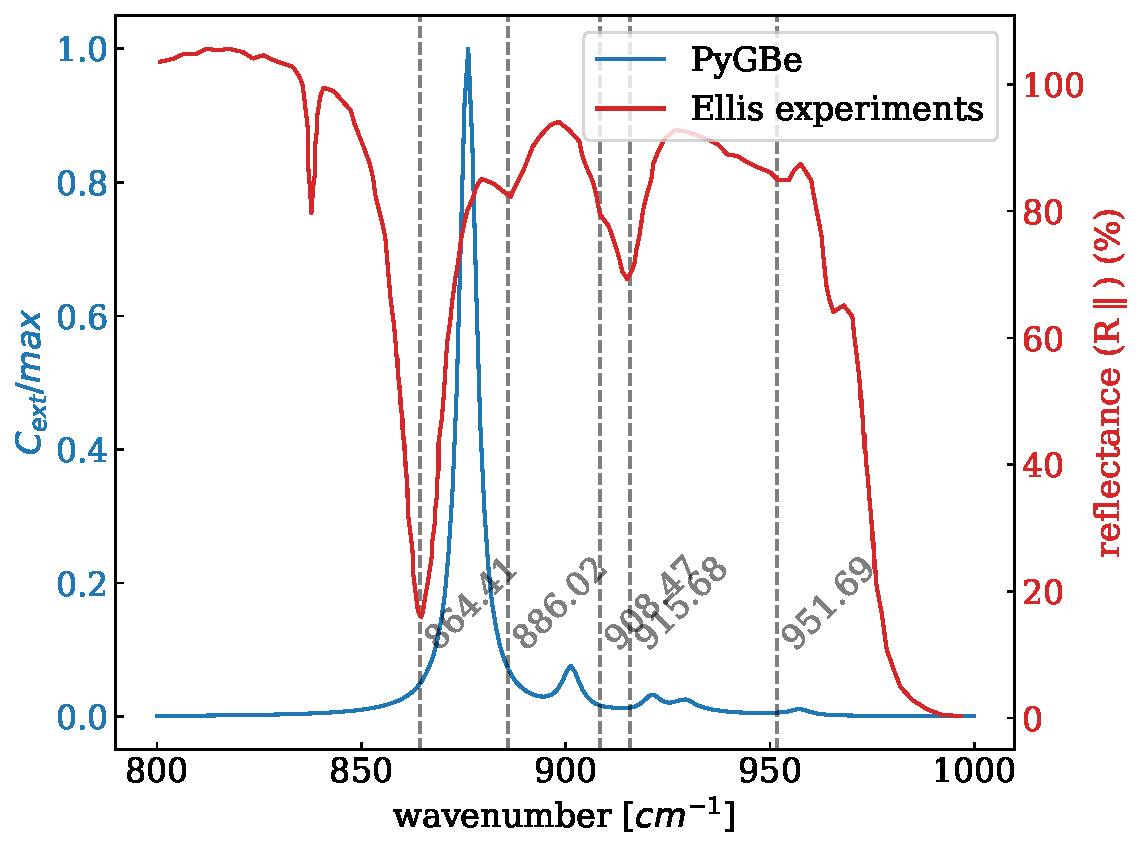
\includegraphics[width=0.85\textwidth]{pygbe_vs_exp_fig2a_Ellis.pdf} 
    \caption{\pygbe vs.\ the experiments presented in Figure 2a of Ellis et al., 2016 (we obtained the data 
    digitizing by hand from their figure using WebPlotDigitizer).}
    \label{fig:pygbe_vs_exp_2a}
 \end{figure}

\paragraph{First-order correction.}

Since our simulations do not take into account coupling effects in an array of prisms, we cannot strictly match 
the conditions to validate our solver. However, from Figure S4 in the supplementary 
materials of Ellis et al., we know that coupling effects affect the $E^{\parallel}_{100}$ 
mode by a shift of 12.17 cm$^{-1}$. Therefore, as a \textit{first-order correction} we can 
subtract this amount from our simulations to account for coupling effects. In Figure 
\ref{fig:val_2a}, we present the result after applying this correction for coupling effects.
It is worth mentioning that the far-left (837 cm$^{-1}$) and far-right (964 cm$^{-1}$) peaks 
on the results of Ellis et al., are peaks associated with zone-folded LO (longitudinal) phonons of 4H-SiC,
an effect they say is beyond the scope of their analysis \cite{ellis2016}. They concentrate their analysis on the peaks that occur between 864 and 961 cm$^{-1}$.
If we use the same approximation and compare the results with the simulations of Ellis et al.\ on
Figure 2 of their paper (green curve), we obtain Figure \ref{fig:rep_2a}.

\begin{figure}
    \centering
    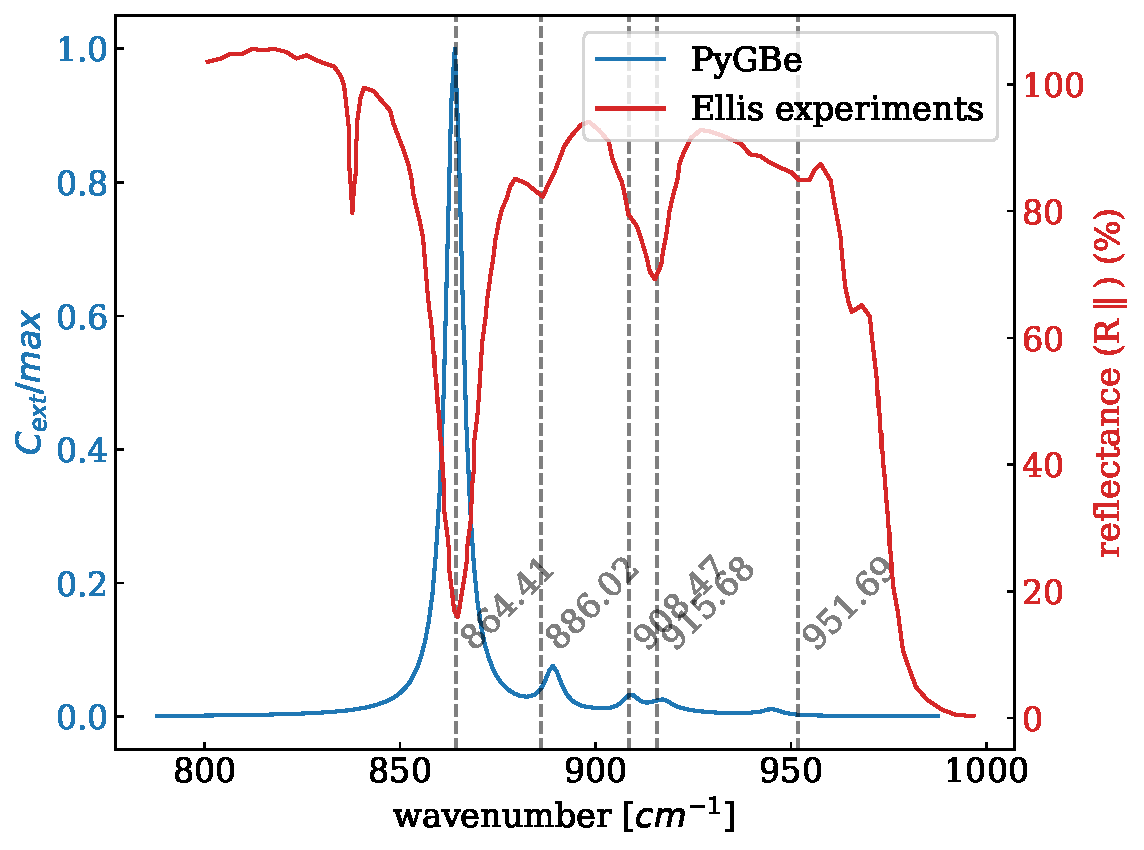
\includegraphics[width=0.85\textwidth]{validation_FOA_fig2a_Ellis.pdf} 
    \caption{Validation against experiments in Figure 2a of Ellis, et al., 2016, using the first-order correction, as explained in the text.}
    \label{fig:val_2a}
 \end{figure}

\begin{figure}
    \centering
    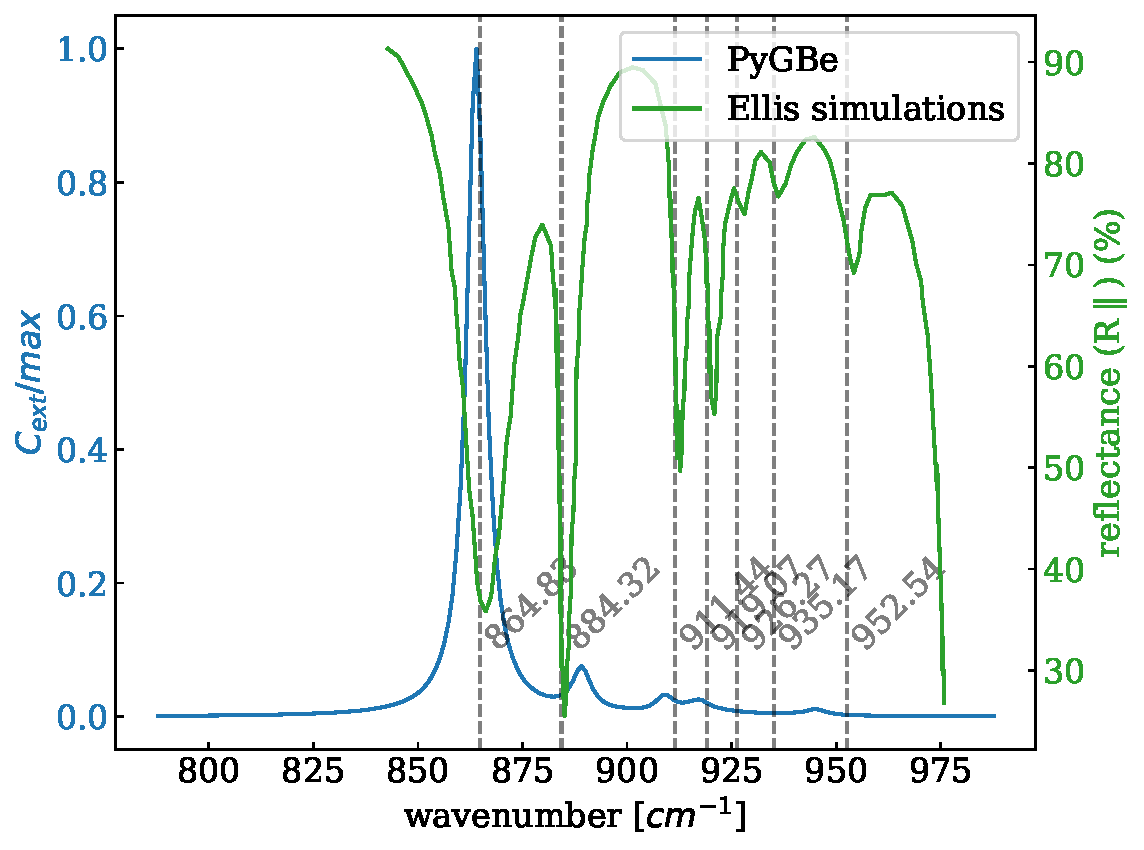
\includegraphics[width=0.85\textwidth]{replication_FOA_fig2a_Ellis.pdf} 
    \caption{Replication of the simulations in Figure 2a of Ellis et al., 2016, using the first-order correction, as explained in the text.}
    \label{fig:rep_2a}
 \end{figure}
 
 
 \subsection{Reproducibility and data management} \label{sec:reprod}
 
 Barba (2019) describes the elements of reproducible computational research that we have adopted in our practice \cite{barba2019praxis}. 
 A key element is professional software management and engineering, and the central technology solution is version control. 
 Preserving a complete history of changes is the only way to manage complex software projects that can support reproducibility. 
 Moreover, all our research software is developed in the open, and shared under permissive public licenses, such as BSD-3 or MIT License. 
 These open licenses permit all uses, as well as derivative works, only subject to attribution.
 Another key element of transparent and reproducible computational modeling is \emph{automation}.
Automating every step means \emph{turning protocols into code.}
For example, simulations are launched with parameters fed from a configuration file rather than an interactive prompt, and all figures and plots are produced by writing scripts, rather than pointing-and-clicking on a graphical interface. 
The goal is to create complete ``recipes'' in code, which can be run, versioned, and shared. 

Our signature reproducibility practice is to organize and share in an archival-quality repository (providing a global identifier) all digital artifacts associated with the results in the paper. 
This includes input files, configuration files, post-processing scripts, files specifying the build process and containerization (e.g., Docker files), and even cloud computing machine definitions, if applicable \cite{mesnard-barba2019}.
We call these openly shared file sets \emph{reproducibility packages}, or repro-packs for short, and we have been doing this for many years and improving the process iteratively. 
The basic steps were already contained in the ``Reproducibility PI Manifesto'' of 2012 \cite{barba2012manifesto}, where Barba pledged to always share a manuscript's data, plotting scripts and figures under CC-BY (Creative Commons Attribution license).
Notably, this makes the figures re-usable by readers, without requiring them to ask permissions from the publisher, even if there was a transfer of copyright of the paper (the figures are included in the paper under the conditions of the public license). 
We later extended the practice to include all other digital artifacts associated with the results, beyond secondary data and figures. 
As in our previous papers, readers can reproduce all the figures in this paper using the repro-packs shared in the manuscript GitHub repository, and archived separately in Zenodo. 
They include Jupyter notebooks with all the plotting code, and also the manually digitized data from the figures in the source articles for our replication cases.
Barba and Thiruvathukal, 2017 \cite{BarbaThiruvathukal2017}, explain that it is \emph{not enough} to provide these materials in a GitHub repository (the owner of a repository is always able to delete it), and one should deposit the reproducibility packages in an archival service providing a global identifier and permanent link (like a digital object identifier, DOI).
%[LIST, EXPLAIN, CITE ARCHIVES] 

The following items of archived digital artifacts accompany this paper:

\begin{compactitem}

\item[$\triangleright$] The software repository for \pygbe is at \href{https://github.com/barbagroup/pygbe}{https://github.com/barbagroup/pygbe}.

\item[$\triangleright$] The repository for this paper is at \href{https://github.com/barbagroup/pygbe_validation_paper}{https://github.com/barbagroup/pygbe\_validation\_paper}, which also includes the manuscript source files in LaTeX.

\item[$\triangleright$] The problem datasets for replication of Rockstuhl et al., 2005, are in the manuscript repository, but also archived in Zenodo  at \href{https://doi.org/10.5281/zenodo.3962534}{10.5281/zenodo.3962534}  \cite{ClementiBarba2020-Zen_a}.

\item[$\triangleright$] Execution files for all runs are archived in Zenodo at \href{https://doi.org/10.5281/zenodo.3962576}{10.5281/zenodo.3962576} \cite{ClementiBarba2020-Zen_b}.

\item[$\triangleright$] The problem datasets for validation and replication of results from Ellis et al., 2016 are archived in Zenodo at \href{https://doi.org/10.5281/zenodo.3962584}{10.5281/zenodo.3962584}\cite{ClementiBarba2020-Zen_c}.

\item[$\triangleright$] The file sets for reproducing the figures for the replication of results from Rockstuhl et al., 2005 are archived in Zenodo at \href{https://doi.org/10.5281/zenodo. 3962791}{10.5281/zenodo. 3962791} \cite{ClementiBarba2020-Zen_d}.

\item[$\triangleright$] The file sets for reproducing the figures for the validation and replication of results from Ellis et al., 2017 are arhived in Zenodo at \href{https://doi.org/3962797/zenodo.3962791}{10.5281/zenodo.3962797} \cite{ClementiBarba2020-Zen_e}.

\end{compactitem}



\section{Discussion}\label{sec:discussion}


\newpage
\bibliographystyle{vancouver}
\bibliography{pygbe_rep_val} %don't leave spaces between elements, it throws error


\end{document}